\begin{definition}[Stückweise Regularität]
Eine Kurve $C\coloneqq\varphi([a,b])\subset\mathbb{R}^n$ mit 
stetiger Parametrisierung $\varphi:[a,b]\rightarrow\mathbb{R}^n$ heißt \textbf{stückweise regulär}, falls es
\begin{equation*}
	a=s_0 < s_1 < ... < s_k = b
\end{equation*}
gibt, so dass
\begin{equation*}
	\varphi((s_{j-1},s_j)=C
\end{equation*}
eine 1-dimensionale Mannigfaltigkeit ist. Ohne Beschränkung der 
Allgemeinheit setzten wir dann $\varphi$ als zugehörige 
Parametrisierung auf $(s_{j-1},s_j)$. Die Abbildung 
\begin{equation*}
	t:C_j\rightarrow\mathbb{R}^n \ \ \ 
	\mathrm{mit\ }t(\varphi(s)=
	\frac{\varphi'(s)}{|\varphi'(s)|}	
\end{equation*}
stellt dann die Einheitstangente dar.
\begin{center}
	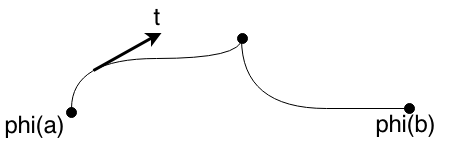
\includegraphics[scale=0.5]{pictures/010-01.png}
\end{center}
\end{definition}

\begin{definition}[Geschlossene Kurven]
Eine Kurve $C\coloneqq\varphi([a,b])$ heißt \textbf{geschlossen}, 
wenn $\varphi(a)=\varphi(b)$ ist.
\begin{center}
	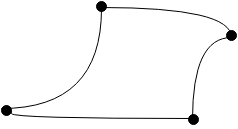
\includegraphics[scale=0.5]{pictures/010-02.png}
\end{center}
Wir schreiben dann ''$-C$'' für die zu $C$ entgegengesetzt laufende 
Kurve und ''$C_1+C_2$'' für zusammengesetzte Kurven, wenn $C=C_1+C_2$ stückweise regulär ist.
\begin{center}
	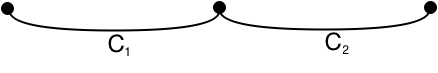
\includegraphics[scale=0.5]{pictures/010-02_1.png}
\end{center}
Das Integral entlang der Kurve ist dann
\begin{equation*}
	\int_CF(x)\cdot t(x)\mathrm{d}a
\end{equation*}
Offenbar ist 
\begin{equation}
	\int_CF(x)\cdot t(x)\mathrm{d}a = 
	\int_a^b F(\varphi(s))\cdot\frac{\varphi'(s)}{|\varphi'(s)|}
	|\varphi'(s)|\mathrm{d}s = 
	\int_a^b F(\varphi(s))\varphi'(s)\mathrm{d}s
\end{equation}
\end{definition}
\newpage
\begin{satz}
Sei $F:\Omega\subset\mathbb{R}^n\rightarrow\mathbb{R}^n$ stetig 
auf dem (offen zusammenhängenden) Gebiet $\Omega$. Dann sind 
folgende Behauptung äquivalent:
\begin{enumerate}
	\item 	$F$ ist ein Gradientenfeld
	\item 	Das Integral verschwindet auf geschlossenen 
			Kurven.
			\begin{equation}
					\int_C F(x)\cdot t(x)\mathrm{d}a = 0
			\end{equation}
	\item 	Das Integral ist wegunabhängig, das heißt
			\begin{equation}
					\int_{C_1} F(x)\cdot t(x)\mathrm{d}a = 
					\int_{C_2} F(x)\cdot t(x)\mathrm{d}a
			\end{equation}
			für stückweise reguläre Kurven $C_1$ und $C_2$ 
			mit $\varphi_1(a)=\varphi_2(a)$ und 
			$\varphi_1(b)=\varphi_2(b)$.
\end{enumerate}
\end{satz}

\begin{proof}
Sei $F=f'$ für ein $f\in C^1(\Omega)$ und $C$ eine 
geschlossene, stückweise reguläre Kurve mit der Parametrisierung 
$\varphi$. Dann 
\begin{equation*}
	\int_C F(x)\cdot t(x)\mathrm{d}a \stackrel{(33.2)}{=} 
	\int_a^b \diff{}{s}f(\varphi(s))\mathrm{d}s 			
	\stackrel{\mathrm{Haups.}}{=} 
	f(\varphi(b)) - f(\varphi(a)) = 0 
	\tag{$\#$}
\end{equation*}
Daraus folgt sofort (33.3).\\ 
Um nun (33.4) zu zeigen, nehmen wir 
an, dass (33.3) gilt und setzen $\tilde{x},x\Omega$ und $C_1, 
C_2$ als zwei Kurven mit $\varphi_1(a) = \varphi_2(a) =
 \tilde{x}$ und $\varphi_1(a) = \varphi_2(b) = x$.
\begin{center}
	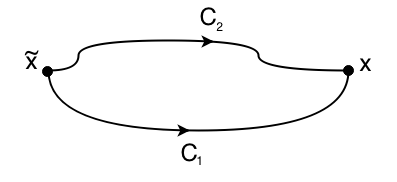
\includegraphics[scale=0.5]{pictures/010-03.png}
\end{center}
Dann setzen wir als Parametrisierung für $C=C_1-C_2$
\begin{equation*}
	\psi(s)\coloneqq\left\{\begin{array}{ll}
	\varphi_1(s) &  \ \ t\in(a,b) \\
	\varphi_2(2b-s) & \ \ t\in(b,2b-a)
	\end{array}\right.
\end{equation*}
Da $C$ geschlossen ist, ergibt sich
\begin{equation*}
	0 = \int_C F(x)\cdot t(x)\mathrm{d}a = 
	\int_{C_1} F(x)\cdot t(x)\mathrm{d}a + 
	\int_{-C_2} F(x)\cdot t(x)\mathrm{d}a = 
\end{equation*}
\begin{equation*}
	= \int_{C_1} F(x)\cdot t(x)\mathrm{d}a - 
	\int_{C_2} F(x)\cdot t(x)\mathrm{d}a = 0
\end{equation*}
Damit folgt (33.4).\\
Gelte nun (33.4) und wir fixieren ein $\tilde{x}\in\Omega$. 
Weiterhin sei $C$ eine Kurve mit $\varphi(a)=\tilde{x}$ und 
$\varphi(b)=x$. Nach (33.4) ist dann folgendes $f$ für alle 
$x\in\Omega$ wohldefiniert:
\begin{equation*}
	f(x)\coloneqq\int_CF(x)\cdot t(x)\mathrm{d}a
	\tag{$\dagger$}
\end{equation*}
Nun sei für ein festes $x\in\Omega$
\begin{equation*}
	\varphi(\tau)=x+\tau e_j
\end{equation*}
\begin{equation*}
	C(s)\coloneqq\varphi([b,s])
\end{equation*}
Daraus folgt dann
\begin{equation*}
	\frac{1}{2}\left(f(x+se_j)-f(x)\right) 
	\stackrel{(\dagger)}{=} 
	\frac{1}{s}\int_{C(s)}F(x)\cdot t(x)\mathrm{d}a 
	\stackrel{(33.2)}{=}  
	\frac{1}{s}\int_0^s F(\varphi(t))\cdot e_j\mathrm{d}\tau = 
\end{equation*}
\begin{equation*}
	\stackrel{\mathrm{MWS}}{=} 
	\frac{1}{2}F(\varphi(\tilde{s})e_js
\end{equation*}
für ein festes $\tilde{s}\in(0,s)$. Machen wir nun den 
Grenzprozess $s\rightarrow 0$, so folgt
\begin{equation*}
	\pdiff{}{x_j}f=F(x)e_j=F^j(x)
\end{equation*}
Damit ist $F=f'$ und $f\in C^1$. 
\end{proof}
\newpage
\begin{satz}
Sei $F:\Omega\subset\mathbb{R}^n\rightarrow\mathbb{R}^n$ ein 
Gradientenfeld mit $F=f'$, wobei $f$ stetig differenzierbar auf 
dem Gebiet $\Omega$ ist. Außerdem sei $x_0\in\Omega$ und 
$\varphi:[a,b]\rightarrow\Omega$ eine stückweise reguläre Kurve 
mit $\varphi(a)=x_0$ und $\varphi(b)=x$. Dann gilt
\begin{equation*}
	f(x)=f(x_0)+\int_{\varphi([a,b])} F(x)\cdot t(x) \mathrm{d}a
	\stackrel{(33.2)}{=} 
	f(x_0)+\int_a^b F(\varphi(s)\varphi'(s)\mathrm{d}s
\end{equation*}
\emph{Anmerkung:} Jede Wahl von $x_0$ liefert eine 
Stammfunktion.
\end{satz}

\begin{definition}[Zusammenziehbarkeit]
Eine geschlossene Kurve $C\coloneqq\varphi([a,b])\subset\Omega$ 
heißt \textbf{zusammenziehbar} auf einen Punkt in $\Omega$, 
falls eine stetige Abbildung $h:[a,b]\times[0,1]\rightarrow\Omega$ existiert, die folgende Bedingungen erfüllt:
\begin{enumerate}
	\item $h(\tau,0)=\varphi(\tau),\ h(\tau,1)=x_0 \ \ \forall
			\tau\in[0,1]$
	\item $h(a,s)=h(b,s) \ \ \forall s\in[0,1]$
\end{enumerate}
\begin{center}
	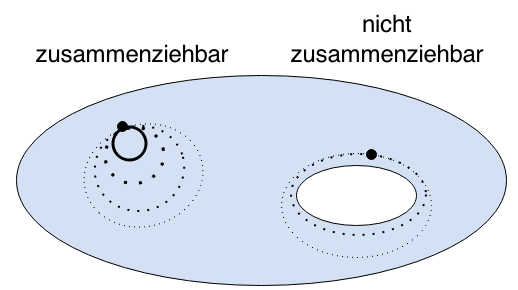
\includegraphics[scale=0.5]{pictures/010-04.png}
\end{center}
\end{definition}

\begin{definition}[Einfacherer Zusammenhang]
Ein Gebiet $\Omega$ heißt \textbf{einfach zusammenhängend}, 
falls jede geschlossene Kurve auf einen Punkt in $\Omega$ 
zusammenziehbar ist.
\end{definition}

\begin{satz}
Sei $F:\Omega\subset\mathbb{R}^n\rightarrow\mathbb{R}^n$ ein 
stetig differenzierbares Vektorfeld auf dem einfach 
zusammenhängenden $\Omega$. Dann gilt:\\
$F$ ist \emph{genau dann} ein Gradientenfeld, wenn die 
Integrabilitätsbedingung aus (33.1) erfüllt ist.
\end{satz}

\begin{proof}
Die Hinrichtung wurde für Satz 33.1 bereits bewiesen. Für die 
Rückrichtung zeigen wir, dass $\int_CF\cdot t\ \mathrm{d}a = 0$ für alle geschlossenen, stückweise regulären Kurven. Mit Satz 33.2 folgt dann die Behauptung.
\end{proof}

\begin{beispiel}
Sei $F:\Omega\subset\mathbb{R}^2\setminus{0}\rightarrow\mathbb{R}^2$ mit
\begin{equation*}
	F(x)=\left(	-\frac{x_2}{|x|^2},\ \frac{x_2}{|x|^2 }\right)
\end{equation*}
Die Integrabilitätsbedingung ist erfüllt, es gilt also
\begin{equation*}
	\pdiff{}{x_2}F^1=\pdiff{}{x_1}F^2 \ \ \ 
	\left(=\frac{x_2^2+x_1^2}{|x|^4}\right)
\end{equation*}
Betrachten wir nun die geschlossene Kurve $C\coloneqq 
\varphi([0,2\pi])$ mit $\varphi(t)=(r\cos t,\ r\sin t)$. 
Dann ist das Integral
\begin{equation*}
	\int_C F(x)\cdot t(x)\mathrm{d}t = 
	\int_0^{2\pi}F(\varphi(t))\cdot\varphi'(t)\mathrm{d}t = 
	\frac{1}{r^2}\int_0^{2\pi}\begin{pmatrix}
	-r\sin t \\ r\cos t	\end{pmatrix} \cdot 
	\begin{pmatrix}
	-r\sin t \\ r\cos t	\end{pmatrix}\mathrm{d}t = 
\end{equation*}
\begin{equation*}
	= \int_0^{2\pi}\mathrm{d}t = 2\pi \neq 0
\end{equation*}
Das geschlossene Kurvenintegral ist also nicht null. Das liegt 
daran, dass $F$ kein Gradientenfeld ist. Es besitzt nämlich 
eine Singularität im Ursprung.
\end{beispiel}

\chapter{Gewöhnliche Differenzialgleichungen}

\section{Einführung}
Eine \textbf{Differenzialgleichung} ist eine Gleichung, in der 
unbekannte Funktionen, deren Ableitungen und deren Argumente 
auftreten, wie z.B.
\begin{equation*}
	u(x)-x=u \ \ \mathrm{oder\ \ } u''(x) = x
\end{equation*}
Das Ziel unserer Überlegungen wird also sein müssen, 
herauszufinden, welche $u:\mathbb{R}\rightarrow\mathbb{R}$ 
zumindest auf einem Intervall $I\subset\mathbb{R}$ solche 
Gleichungen lösen. Insbesondere müssen dabei alle 
auftretenden Ableitungen existieren.\\
\linebreak
Falls die gesuchte Funktion $u$ nur von einem Argument 
$x\in\mathbb{R}$ abhängt, so spricht man von einer 
\textbf{gewöhnlichen Differenzialgleichung}, die 
implizit durch
\begin{equation*}
	f\left(x,u(x),u'(x),...,u^{(k)}(x)\right)=0
\end{equation*}
oder explizit durch
\begin{equation*}
	u^{(k)}(x)=f\left(x,u(x),u'(x),...,u^{(k-1)}(x)\right)
\end{equation*}
gegeben sein kann. Ist die k-te Ableitung die höchste, so spricht man von einer Differenzialgleichung k-ter Ordnung. 
Hängt sie von mehreren Argumenten ab, so nennt man sie 
\textbf{partiell}.\\
\linebreak
Sind mehrere unbekannte Funktionen gesucht, die auch 
gekoppelt sein können, so spricht man von einem \textbf{System 
von Differenzialgleichungen}. \newpage
\begin{equation*}
	u'(x)=v(x)
\end{equation*}
\begin{equation*}
	v'(x)=u(x)
\end{equation*}
\linebreak
Es stellt sich natürlich die Frage, wo Differenzialgleichungen 
Anwendung finden:\\
\linebreak
\textbf{a. Mathematische Rätsel}\\
\linebreak
Man nehme sich eine bekannte Funktion her, differenziere sie so
oft wie möglich oder nötig und leite daraus eine 
Differenzialgleichung her.
\begin{eqnarray*}
u(x)\coloneqq e^x & \Rightarrow & u'-u=0 \ \ \mathrm{oder\ \ } u''-u = 0 \\ 
u(x)\coloneqq x^2 & \Rightarrow & xu'-2u=0 \ \ \mathrm{oder\ \ } u''-u = 0 \\
u(x)\coloneqq -\frac{1}{x} & \Rightarrow & u'-u^2=0 \ \ \mathrm{oder\ \ } u''-2u^3 = 0 \\
\end{eqnarray*}
Solche Gleichungen zu lösen, kann sehr anstrengend sein. 
Die letzte Gleichung hat zum Beispiel nicht mal eine Lösung 
auf der reellen Achse!\\
\linebreak
\textbf{b. Prozesse in Natur und Technik}\\
\linebreak
Das Studium von Differenzialgleichungen ist fundamental für 
Anwendungen in Mathematik, Naturwissenschaften, Technik und 
Ökonomie. Hier findet sich ein blendendes Beispiel dafür, 
wie sich Mathematik und Naturwissenschaften gegenseitig 
befruchtet haben. \\
Das Grundprinzip ist immer dasselbe: Eine Differenzialgleichung 
beschreibt ein Naturgesetz \emph{im kleinen}, wohingegen die 
Lösung derselben den eigentlichen Naturvorgang \emph{im großen} 
beschreibt.\\
\linebreak
\begin{beispiel}[Exponentielles Wachstum]
Sei $u(t)$ die Größe einer Population (Bakterien, Bevölkerung) 
als Funktion der Zeit $t$. Nach der Zeitspanne $\Delta t$ 
verzeichnen wir den Zuwachs
\begin{equation*}
\Delta u = u(t+\Delta t) - u(t)
\end{equation*}
Diese Erkenntnis bietet jedoch von Innen heraus noch keine 
Aussage. Deshalb muss an dieser Stelle eine 
 \textbf{Modellannahme}, ein Naturgesetz, den nötigen Ansatz 
liefern: Die Erfahrung zeigt, dass $\Delta u$ für kleine 
$\Delta t$ proportional zu $\Delta t$ ist. \\
In mathematischer Form heißt das 
\begin{equation*}
\Delta u=\alpha u \Delta t
\end{equation*}
\begin{equation*}
\frac{\Delta u}{ \Delta t}
=\alpha u
\end{equation*}
Wobei $\alpha$ ein zunächst beliebiger Proportionalitätsfaktor 
ist. Machen wir nun den Grenzprozess $\Delta t \rightarrow 0$, so erhalten wir 
\begin{equation*}
u'=\alpha u
\end{equation*}
Diese Differenzialgleichung spiegelt unsere Modellannahme wieder 
und besitzt die allgemeine Lösung
\begin{equation*}
u(t)=Ce^{\alpha t}
\end{equation*}
wobei $C$ hier eine Integrationskonstante darstellt, die 
abhängig von den Anfangsbedingungen des Problems ist. Kennen 
wir $u_0\coloneqq u(t=0)$, so erhalten wir
\begin{equation*}
u(t)=u_0e^{\alpha t}
\end{equation*}
Die Wachstumsrate $\alpha$ kann auch als Differenz aus 
Geburtenrate $\gamma$ und Todesrate $\tau$ aufgefasst werden. 
\begin{equation*}
u'=\gamma u -\tau u
\end{equation*}
Im Spezialfall, dass $\gamma=0$ ist, erhalten wir eine 
Population, in der es nur Todesfälle gibt. Ein Beispiel 
dafür wäre der radioaktive Zerfall.
\end{beispiel}
